% File generato da main.py: tabelle e grafici per la relazione
% Richiede \usepackage{float} e \usepackage{graphicx}

\begin{table}[H]
    \centering
    \begin{tabular}{c|c|c|c}
      \# & $N$ & $NT$ [s] & $T$ [s] \\
      \hline
      1 & 10 & 16.23 & 1.623 \\
      2 & 10 & 16.41 & 1.641 \\
      3 & 10 & 16.51 & 1.651 \\
      4 & 10 & 16.30 & 1.630 \\
      5 & 10 & 16.47 & 1.647 \\
      6 & 10 & 16.39 & 1.639 \\
    \end{tabular}
    \caption{Misure $d_1$ = (482.3 $\pm$ 0.5) mm}
    \label{tab:misure_d1}
\end{table}

\begin{table}[H]
    \centering
    \begin{tabular}{c|c|c|c}
      \# & $N$ & $NT$ [s] & $T$ [s] \\
      \hline
      1 & 10 & 15.70 & 1.570 \\
      2 & 10 & 15.83 & 1.583 \\
      3 & 10 & 15.74 & 1.574 \\
      4 & 10 & 15.84 & 1.584 \\
      5 & 10 & 15.80 & 1.580 \\
    \end{tabular}
    \caption{Misure $d_2$ = (375.2 $\pm$ 0.5) mm}
    \label{tab:misure_d2}
\end{table}

\begin{table}[H]
    \centering
    \begin{tabular}{c|c|c|c}
      \# & $N$ & $NT$ [s] & $T$ [s] \\
      \hline
      1 & 10 & 15.77 & 1.577 \\
      2 & 10 & 15.72 & 1.572 \\
      3 & 10 & 15.65 & 1.565 \\
      4 & 10 & 15.73 & 1.573 \\
      5 & 10 & 15.74 & 1.574 \\
    \end{tabular}
    \caption{Misure $d_3$ = (276.1 $\pm$ 1.2) mm}
    \label{tab:misure_d3}
\end{table}

\begin{table}[H]
    \centering
    \begin{tabular}{c|c|c|c}
      \# & $N$ & $NT$ [s] & $T$ [s] \\
      \hline
      1 & 10 & 16.83 & 1.683 \\
      2 & 10 & 16.80 & 1.680 \\
      3 & 10 & 16.83 & 1.683 \\
      4 & 10 & 16.77 & 1.677 \\
      5 & 10 & 16.90 & 1.690 \\
    \end{tabular}
    \caption{Misure $d_4$ = (176.0 $\pm$ 1.2) mm}
    \label{tab:misure_d4}
\end{table}

\begin{table}[H]
    \centering
    \begin{tabular}{c|c|c|c}
      \# & $N$ & $NT$ [s] & $T$ [s] \\
      \hline
      1 & 10 & 22.93 & 2.293 \\
      2 & 10 & 22.95 & 2.295 \\
      3 & 10 & 22.90 & 2.290 \\
      4 & 10 & 22.97 & 2.297 \\
      5 & 10 & 22.92 & 2.292 \\
    \end{tabular}
    \caption{Misure $d_5$ = (75.1 $\pm$ 1.2) mm}
    \label{tab:misure_d5}
\end{table}

\begin{table}[H]
    \centering
    \begin{tabular}{c|c|c|c}
       & $d$ [mm] & $T$ [s] & residuo [ms] \\
      \hline
      d1 & $482.3 \pm 0.5$ & $1.6385 \pm 0.0044$ & $-9.0 \pm 4.4$ \\
      d2 & $375.2 \pm 0.5$ & $1.5782 \pm 0.0029$ & $-4.0 \pm 2.9$ \\
      d3 & $276.1 \pm 1.2$ & $1.5722 \pm 0.0022$ & $+3.5 \pm 2.2$ \\
      d4 & $176.0 \pm 1.2$ & $1.6826 \pm 0.0024$ & $+1.8 \pm 2.4$ \\
      d5 & $75.1 \pm 1.2$ & $2.2934 \pm 0.0016$ & $-0.5 \pm 1.6$ \\
    \end{tabular}
    \caption{Riepilogo}
    \label{tab:riepilogo}
\end{table}

\begin{table}[H]
    \centering
    \begin{tabular}{c|c}
       & $l$ [mm] \\
      \hline
      best-fit & $1053.6 \pm 0.7$ \\
      misurata & $1051.0 \pm 1.0$ \\
    \end{tabular}
    \caption{Confronto lunghezza asta}
    \label{tab:confronto_l}
\end{table}

\begin{table}[H]
    \centering
    \begin{tabular}{c|c|c}
      $\theta_{\mathrm{eff}}$ & correzione relativa & $\hat{l}$ (mm) \\
      \hline
      8° & 0.12\% & 1052.1 \\
      12° & 0.27\% & 1050.2 \\
      16° & 0.49\% & 1047.6 \\
    \end{tabular}
    \caption{Correzione per ampiezza finita}
    \label{tab:ampiezza}
\end{table}

\begin{figure}[H]
    \centering
    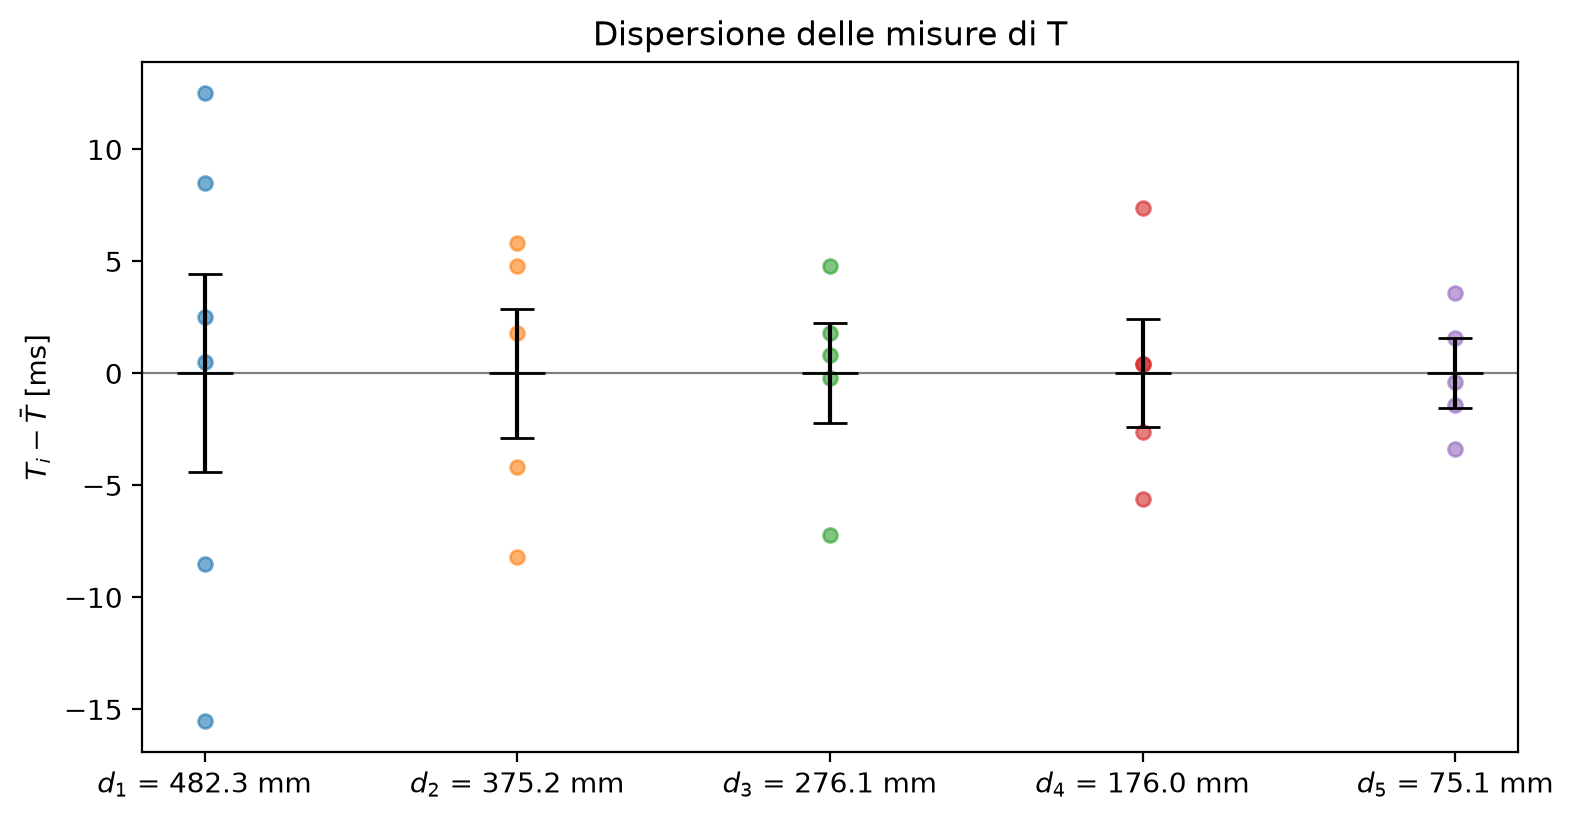
\includegraphics[width=0.9\linewidth]{grafici/disperione_periodo.png}
    \caption{Scarto di ciascuna misura del periodo dalla media del proprio gruppo. Le barre nere indicano l'incertezza $\sigma_T$ sul periodo medio.}
    \label{fig:dispersione}
\end{figure}

\begin{figure}[H]
    \centering
    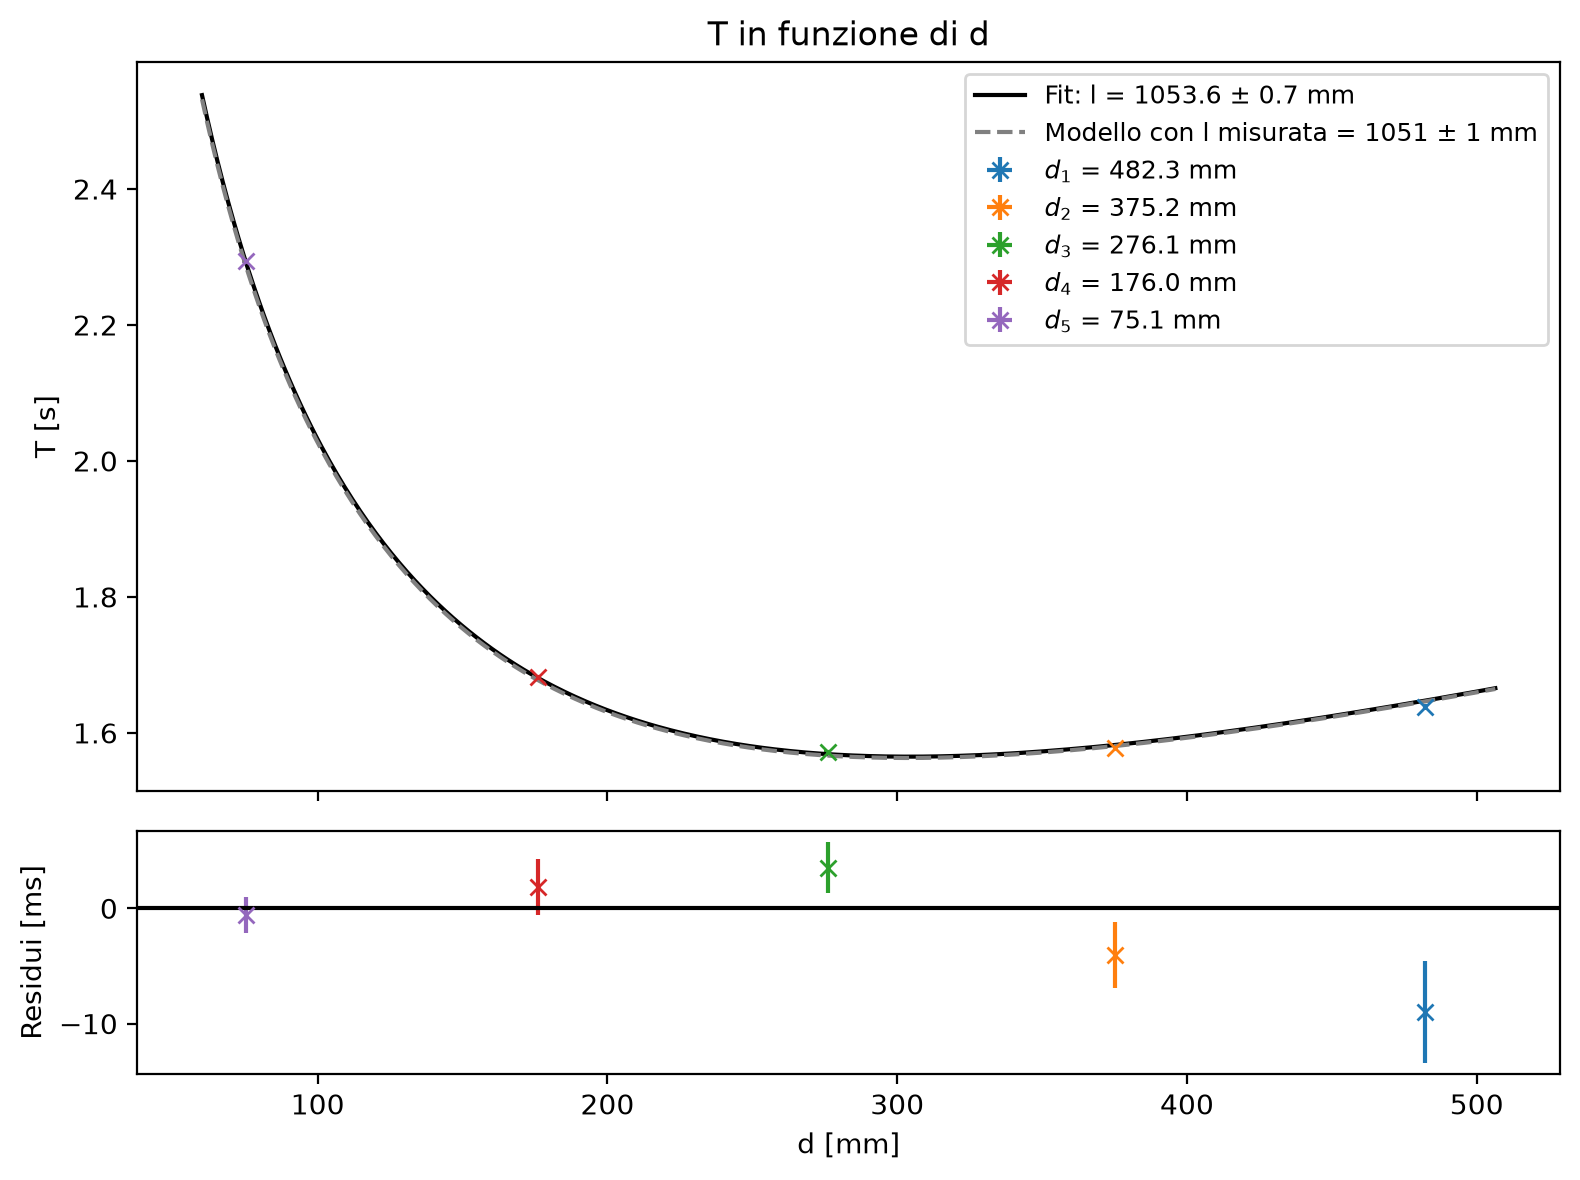
\includegraphics[width=0.8\linewidth]{grafici/fit_periodo.png}
    \caption{In alto: periodo in funzione della distanza $d$, con la curva di best-fit (linea continua) e il modello calcolato con la lunghezza misurata dell'asta (linea tratteggiata). In basso: residui del fit.}
    \label{fig:fit_periodo}
\end{figure}